\item In the interconnection of ideal sources shown in \figref{fig:placeholder_6}, it is known that the $60 V$ source is absorbing power.
\begin{figure}[H]
    \centering
    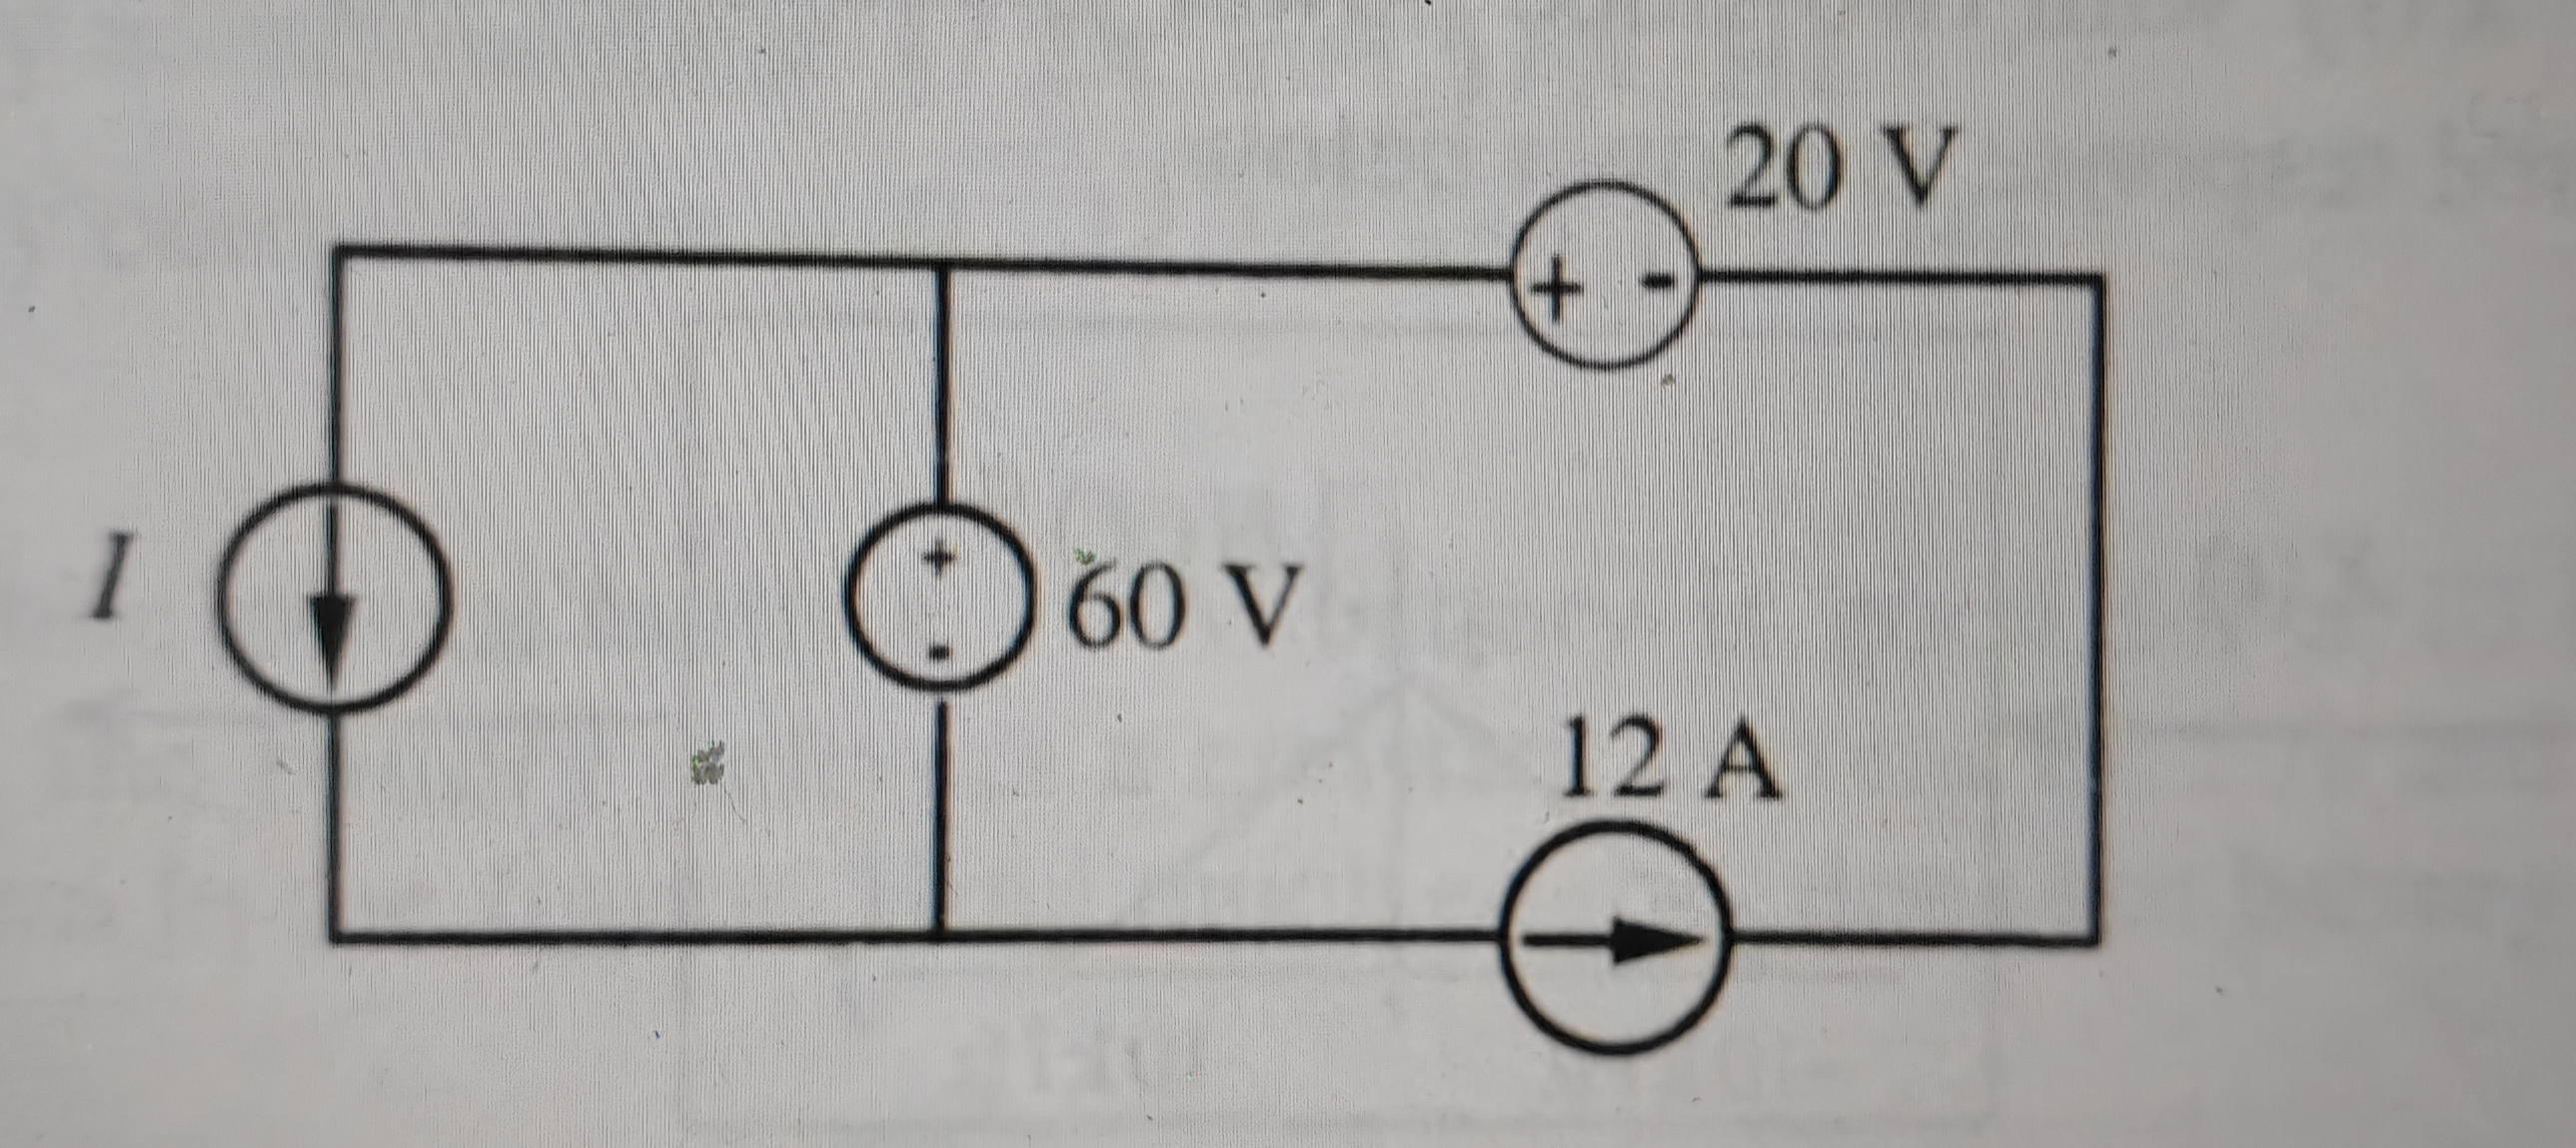
\includegraphics[width=0.7\columnwidth]{GATE/2009/EC/figs/fig_6.jpg}
    \caption{}
    \label{fig:placeholder_6}
\end{figure}
Which of the following can be the value of current source ${I}$ ?

\begin{enumerate}
\begin{multicols}{4}
\item 10 $A$
\item 13 $A$
\item 15 $A$
\item 18 $A$
\end{multicols}
\end{enumerate}
\hfill $\brak{\text{EC 2009}}$

\item In the \figref{fig:placeholder_11} shown below, what value of $R_l$ maximizes the power delivered to $R_l$ ?
\begin{figure}[H]
    \centering
    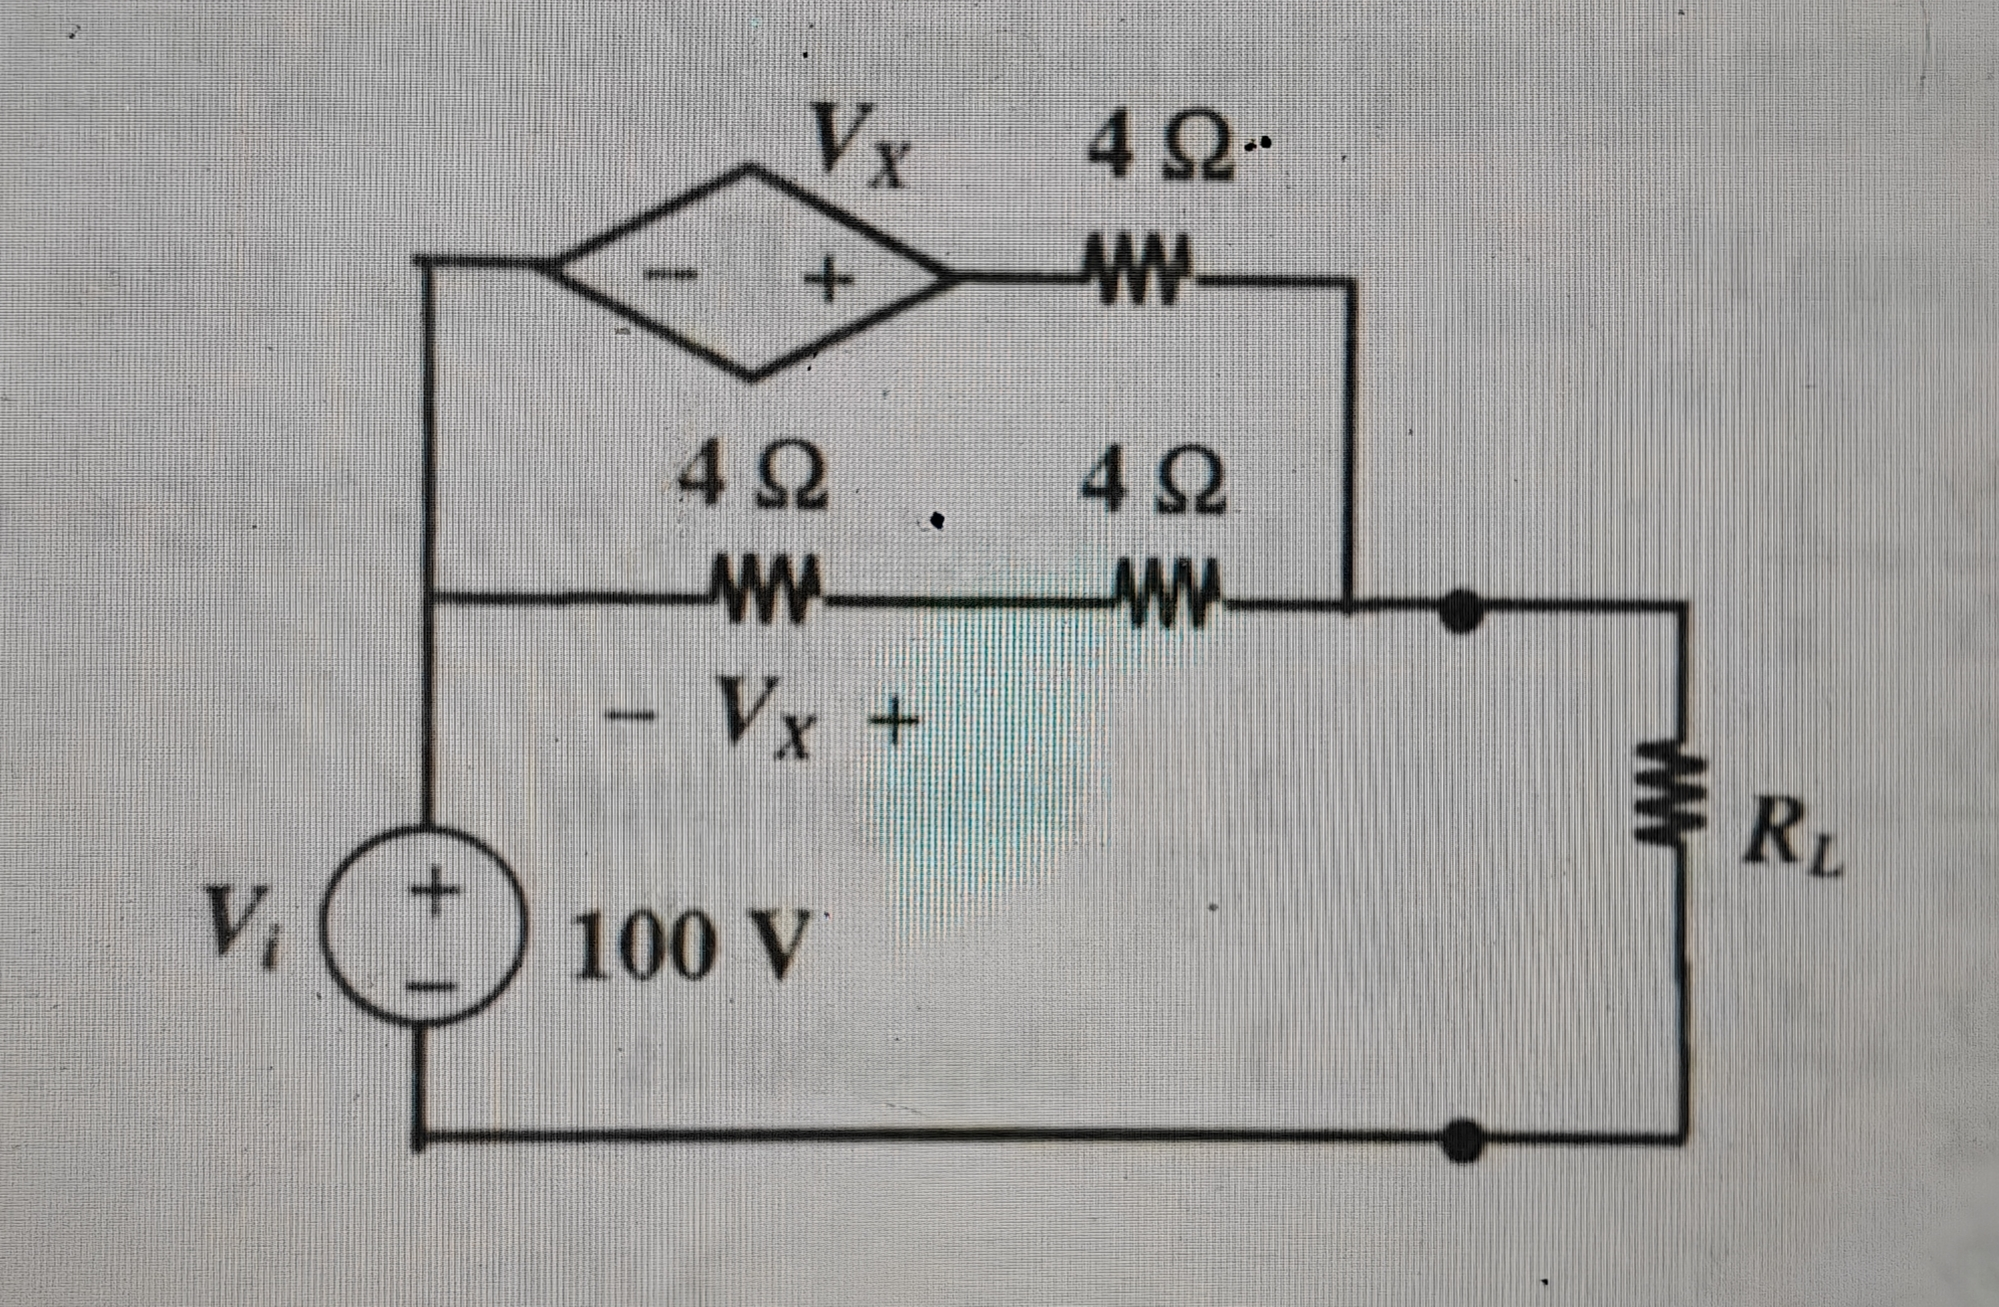
\includegraphics[width=0.7\columnwidth]{GATE/2009/EC/figs/fig_11.jpg}
    \caption{}
    \label{fig:placeholder_11}
\end{figure}
\begin{enumerate}
    \begin{multicols}{4}
        \item $2.4 \ohm$
        \item $\frac{8}{3} \ohm$
        \item $4 \ohm$
        \item $6 \ohm$
    \end{multicols}
\end{enumerate}
\hfill \brak{\text{EC 2009}}

\item The 4-point Discrete Fourier Transform $\brak{DFT}$ of a discrete time sequence $\cbrak{1,0,2,3}$ is 
\begin{enumerate}
    \begin{multicols}{2}
        \item $\sbrak{0,-2+2j, 2,-2,-2j}$
        \item $\sbrak{2,2+2j, 6, 2-2j}$
        \item $\sbrak{6,1-3j, 2, 1+3j}$
        \item $\sbrak{6,-1+3j, 0,-1-3j}$
    
    \end{multicols}
\end{enumerate}
\hfill $\brak{\text{EC 2009}}$

